\documentclass[twocolumn,a4paper]{article}

\title{The importance of beings fractal}
\author{Prof A.~J. Roberts\\
School of Mathematical Sciences\\
University of Adelaide\\
\texttt{mailto:anthony.roberts@adelaide.edu.au}
}

\pagestyle{headings}

\usepackage{graphicx}
%\setlength{\marginparwidth}{6em}

\usepackage[capitalise,nameinlink,noabbrev]{cleveref}
\crefname{equation}{}{}
\crefname{enumi}{}{}


\begin{document}

\maketitle


\begin{quote}
	Good science is the ability to look at things in a new way and 
	achieve an understanding that you didn't have before ... It is opening 
	windows on the world ... you perceive a little tiny glimpse of the way 
	the Universe hangs together, which is a wonderful feeling.  \emph{Hans 
	Kornberg}~\cite{Korny}
\end{quote}

\begin{abstract}
	Fractal geometry, largely inspired by Benoit 
	Mandelbrot~\cite{Mandel} during the sixties and seventies, is one 
	of the great advances in mathematics for two thousand years.  
	Given the rich and diverse power of developments in mathematics 
	and its applications, this is a remarkable claim.  Often presented 
	as being just a part of modern chaos theory, fractals are 
	momentous in their own right.  Euclid's geometry describes the 
	world around us in terms of points, lines and planes---for two 
	thousand years these have formed the somewhat limited repertoire 
	of basic geometric objects with which to describe the universe.  
	\emph{Fractals immeasurably enhance this world-view by providing a 
	description of much around us that is rough and fragmented---of 
	objects that have structure on many sizes.} Examples include: 
	coastlines, rivers, plant distributions, architecture, wind gusts, 
	music, and the cardiovascular system.
\end{abstract}

\tableofcontents

\section{Some fractal models}
\label{sfrac}

Before discussing in detail the common feature of the previously 
mentioned examples, in \cref{sdim}, I present a few examples of 
fractals and the type of physical applications that they have.
%\marginpar{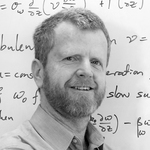
\includegraphics{tonyroberts}}

\subsection{Noise and natural events}
\label{ssnoise}

Have you ever noticed that there are    
\begin{itemize}
	\item  some days where nothing goes right?

	\item  times when you just cannot get a decent telephone connection?

	\item  years when drought follows drought?

	\item  long periods when gusts of wind come thick and fast?
\end{itemize}
That events often occur in bursts 
is a well documented aspect of the world.  The Cantor 
set\footnote{Cantor was a 19th century mathematician interested in 
constructing sets with paradoxical properties.} is a model 
for such bursty phenomena.  
Construct the Cantor set in the following 
manner:
\begin{enumerate}
	\item  start with a bar of some length; 

	\item  then remove its middle third to leave two separate thirds; 

	\item  then remove the middle thirds of these to leave four separate ninths; 

	\item  then remove the middle thirds of these to 
	obtain eight separate twenty-sevenths; 

	\item  and so on.  
\end{enumerate}
Eventually we just 
obtain a scattered dust of points.  However, this dust is specially 
distributed into pairs of points, of pairs of pairs of points, and so 
on.  If the original bar represented a time interval, then the dust 
represents times when events occur and the striking feature is that 
there are long quiescent periods separating the short bursts of 
activity that a clump of the points represents.

\subsection{Coastlines and rivers}
\label{sscoast}

The line of a coast or the path of a river is tortuous.  On a 
small-scale map of Australia or any other country the coastline has 
lots of wriggles.  Upon examining a larger-scale map the wriggles will 
be resolved clearly into gulfs and peninsulas.  However, many smaller 
scale wriggles will still be seen.  These can only be resolved by 
looking at an even larger scale map, whereupon they will be seen to be 
inlets and spits.  But once again there will be wriggles in the 
coast.\footnote{L.~F. Richardson, see \cref{ssturb}, also was 
responsible for recognising these fractal characteristics of 
coastlines.} Similarly for rivers---they exhibit bends and meanders 
upon many scales of length.  The Koch curve models these phenomena.
\begin{figure}
	\centering
    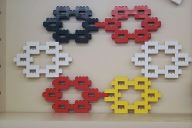
\includegraphics{sflower}
	\caption{the Koch curve is outlined in the middle of this lego `flower', and sequences of transects are classic stages in the formation of the Cantor set.}
	\label{fig:flower}
\end{figure}

Starting with an equilateral triangle, we replace the middle third of 
each side by two segments of the same length (as if we pasted an 
equilateral triangle of one-third the size onto each side); this 
forms the second picture above showing large-scale peninsulas and 
bays.  Repeating this process of extracting the middle third of each 
straight side and replacing it with two segments of the same length, 
the next stage of the construction gives the third picture; it shows 
smaller inlets and spits.  Continually repeating this process leads 
to a very wriggly line that is the Koch curve.  It is perhaps too 
convoluted for a coastline, but on the other hand, it looks far more 
realistic than a routine curve!

\subsection{Turbulence}
\label{ssturb}

Most mathematicians, physicists and engineers would give their right 
arm to understand what is going on in this picture.  It shows 
something of the highly complex motion that is turbulence in a fluid 
as expressed by the following ditty\footnote{This ditty is derived 
from: Big fleas have little fleas upon their backs to bite them, and 
little fleas have lesser fleas, and so on ad infinitum.} by 
L.~F. Richardson~\cite{Rich}:
\begin{verse}
	Big whorls have little whorls,\\
	Which feed on their velocity;\\
	And little whorls have lesser whorls,\\
	and so on to viscosity.
\end{verse}

When air or water moves, a smooth flow quickly breaks up into 
swirling eddies.  These eddies are of a wide range of sizes and, as 
on a windy day, there are often quiescent periods separating the 
various wind gusts.  The structure of turbulence may be epitomised by 
a Sierpinski sponge which is formed from building blocks in much the 
same way as the ``Eiffel tower.''  Form a small unit by putting 20 
blocks face to face along the edges and corners of a $3\times 
3\times 3$ cube, 
leaving the middle of the six faces and the middle of the cube 
vacant.  Make a bigger unit by connecting 20 of these units together 
in the same 
\(
	3\times 3\times 3
\)
 pattern.  And so on to as large a scale as possible.
 
 

\section{Scaling and dimensionality}
\label{sdim}

The common theme in these examples is not just that they have detail 
on many lengths, but also that the structure at any scale is much the 
same at any other scale---the coastline around a continent looks just 
like any small part of the coastline.  If we take a magnifying glass 
or microscope to any of these examples then, no matter what the 
magnification, the geometric detail that we see is the same.  This 
property of looking similar at all scales is termed self-similarity: 
exact in the artificial examples, and statistical or random in 
practical applications.  In order to tease out the self-similar 
characteristics of such objects we need to explore the fractal over 
many lengths and sizes, summarised by equation~\cref{eqf}.  

The coarsest characteristic of fractals is their dimensionality.  
While we normally expect a dimension to be an integer, a natural 
number such as 1, 2 or 3, fractals are best described by means of a 
dimension which is fractional, such as 1.2 or 0.69.  This dimension 
is obtained by blurring the fractal at some size, counting the number 
of blobs in this blurred picture, and then seeing how the count 
varies with the size of the blurring.  Another explanation of this 
process is to count how few ``clumps'' of a certain size the object can 
be broken into, and then see how this count varies with the size of 
the clump.  

\subsection{Points, lines and planes}
\label{seuclid}

Lets become familiar with the argument via some well known geometric 
examples: points, lines, and planes.  Consider a line of some length 
$L$ as shown below.  The line could be curved, but for simplicity 
we take it to be straight.  To ``blur'' the object at a size
\(
	d
\)
I mean that we try to cover as much of the object as possible by discs 
of diameter $d$.  In this picture I have used
\(
	N=9
\)
discs to cover the line segment.  If the discs were half the diameter, 
then we would have to use twice as many of them to cover the line; if 
the discs were one-third the diameter then we would have to use three 
times as many to cover the line; and so on for other sizes.  
Typically, the number of discs needed to cover a line of length $L$ is $N=L/d$.  The important aspect of this relation is that the 
number of discs is inversely proportional to the first power of the 
size (diameter) of the discs: $N\propto d^{-1}$.

Contrast this with what happens when we cover an area $A$ of the 
plane with discs of some diameter $d$:
\(
	N=34
\)
 in the above example.  Typically, 
the number of discs needed to cover an area 
\(
	A
\)
is inversely proportional to the second power of the size of the 
discs: $N\propto d^{-2}$; the number would be close to the area, 
$A$, divided by the area of each disc, $\pi d^2/4$, to be  
\[
	\frac{4A}{\pi d^2}
\]
if it were not for the wastage around the perimeter of 
each disc.

See that the exponent of this relation between $N$, the number of 
discs, and the size of the discs, as measured by the diameter $d$, 
is precisely the dimensionality of the object: a line is 
one-dimensional; an area of the plane is two-dimensional.  This 
relation between the exponent and the dimensionality is true in 
general.  For another example, consider a small number, $n$, of 
points distributed in space---for all
\(
	d
\)
smaller than the minimum separation between the points the number of 
discs needed is precisely the same as the number of points in the set.  
Thus $N=n\times d^0$, and the 0 exponent matches the 
zero-dimensionality of a point or a finite number of points.

For the geometric objects introduced earlier, the relation between $
N$ and $d$ involves a fractional exponent $D$:
\begin{equation}
	N\propto d^{-D}.
	\label{eqf}
\end{equation}
It is only reasonable for us to say that the 
dimensionality of such an object is the fraction $D$.
\begin{table}
	\caption{common Euclidean and fractal objects and their fractal 
	dimension.}
	\label{T:dimens}
	\begin{center}
        \begin{tabular}{lc}
            \hline
            Object & Dimension  \\
            \hline
            point & 0  \\
            Cantor set, \cref{ssnoise} & 0.6309  \\
            line & 1  \\
            Koch curve, \cref{sscoast} & 1.2619  \\
            plane & 2  \\
            Sierpinski sponge, \cref{ssturb} & 2.7268  \\
            solid & 3  \\
            \hline
        \end{tabular}
	\end{center}
\end{table}

\begin{thebibliography}{99}
\addcontentsline{toc}{section}{References}
	\bibitem{Mandel}  B.~B.~Mandelbrot, \emph{The fractal geometry of 
	nature}, 1983.

	\bibitem{Korny}  H.~Kornberg, \emph{J.\ Irreducible Results}.

	\bibitem{Rich} L.~F. Richardson, somewhere and sometime in the 
	1920s.
\end{thebibliography}

\end{document}

